%%%%%%%%%%%%%%%%%%%%%%%%%%%%%%%%%%%%%%%%%%%%%%%%%%%%%%%%%%%%%%%%%%%%%%%%
\section{Results} 
\label{sec:results}
%%%%%%%%%%%%%%%%%%%%%%%%%%%%%%%%%%%%%%%%%%%%%%%%%%%%%%%%%%%%%%%%%%%%%%%%

To compare Caffe SSD performance versus YOLO performance on Jetson TX1, we used their supplied applications for object detection on image files.
We downloaded 600 images from MSCOCO dataset \cite{mscoco}, and measured the total execution time. We made three comparison between the two algorithms: when both run on (1) CPU, (2) GPU without cuDNN, and (3) GPU with cuDNN\footnotemark.

\footnotetext{The NVIDIA CUDA Deep Neural Network library (cuDNN) is a GPU-accelerated library of primitives for deep neural networks. cuDNN provides highly tuned implementations for standard routines such as forward and backward convolution, pooling, normalization, and activation layers.}

Figure \ref{fig:t_exec} shows the execution time of both SSD and YOLO for each of the options described above.
Not surprisingly, running object detection algorithms on a CPU is not as efficient as running them on a GPU. The GPU built-in parallelism is advantageous for such algorithms. \todo{[TODO: comparison between SSD and YOLO on CPU]}

\todo{[TODO: comparison between GPU with and without cuDNN]}

\todo{[TODO: comparison between SSD and YOLO on GPU]}

\begin{figure}[h]
	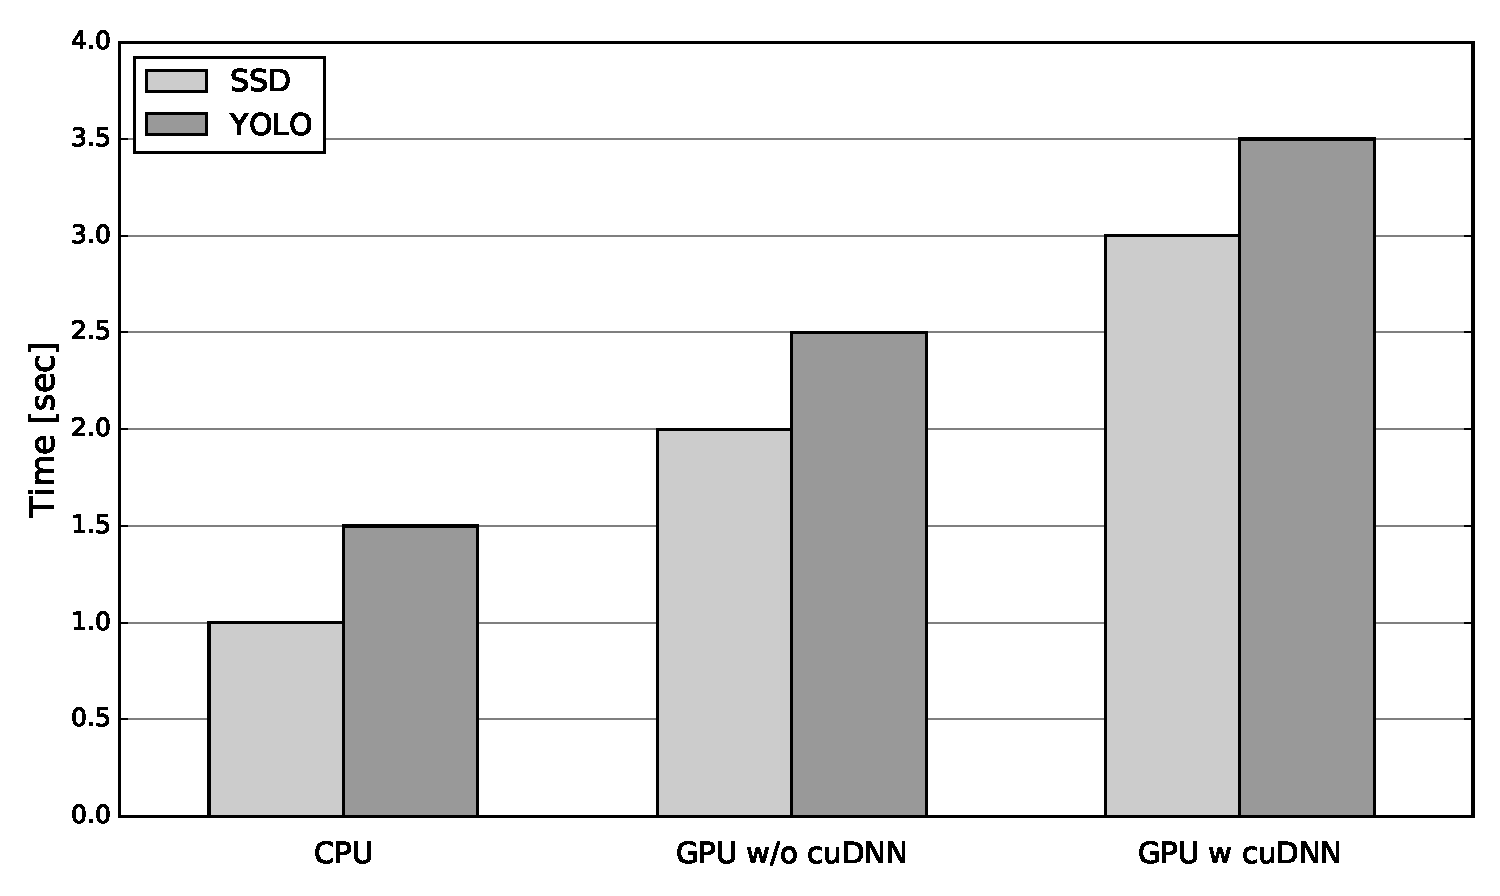
\includegraphics[width=0.48\textwidth]{./imgs/t_exec.pdf}
	\caption{Execution time comparison}
	\label{fig:t_exec}
\end{figure}